\documentclass[12pt, letterpaper]{article}
\usepackage[utf8]{inputenc}
\usepackage[a4paper, total={7in, 10in}]{geometry}
\usepackage{amsmath}
\usepackage{tikz}
\usepackage{pgfplots}

\title{HW 3}
\author{Ben Lirio}
\date{March 8}

\begin{document}
\maketitle
I pledge my honor that I have abided by the Stevens Honor System.
\begin{enumerate}
	\item Flight
		\begin{enumerate}
			\item In order for a flight with $s = 50$ seats to accomadate $k$ passengers who show up, $k \le s$. Let X represent the random variable of the number of passengers who show up, then $P(X \le s)$ is probability all $k$ passengers will have a seat. This can be calculated as follows, $P(X \le 50) = \rho(45) + \rho(46) + \rho(47) + \rho(48) + \rho(49) + \rho(50) = .05 + .1 + .12 + .14 + .25 + .17 = .83$. There is an \textbf{83\%} chance all ticketed passengers who show up will have a seat.
			\item The probability at least one of $k$ passengers who show up will not be seated happens when $k > s$. Which can be shown as $P(X < 50)$ which is the complement to answer 'a'. so $P(X < 50) = 1 - P(X \le 50) = 1 - .83 = .17$. The probability that not all of the $k$ will recieve a seat is \textbf{17\%}.
			\item If you are the first person on standby, then if there must be one free seat on the plane for you to have a seat. This happens when $X \le 49$. So answer derived from a $P(X < 50) = P(X \le 50) - P(X = 50) = .83 - .17 = .66$. If you are the first person on standby there is a \textbf{66\%} you will still be able to fly. Now, if you are the 3rd person on standby $X \le 47$ must be true. $P(X \le 47) = P(45) + P(46) + P(47) = .05 + .10 + .12 = .27$. If you are the third person on standby there is a \textbf{27\%} chance you will still be able to fly.
		\end{enumerate}
	\item Earthquake
		\begin{enumerate}
			\item The probability distrabution of $X$ is \[ \rho(k) = \begin{cases}
			{4\choose k}.25^k.75^{N-k} & 0 \le k \le 4 \\
			0 & otherwise
			\end{cases}
			\]
			\item 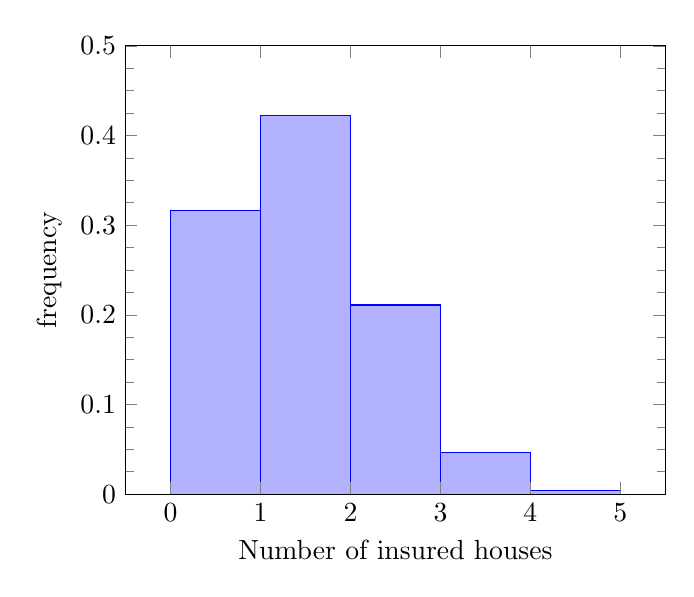
\begin{tikzpicture}
			\begin{axis}[
			ymin=0, ymax=.5,
			minor y tick num = 3,
			area style,
			xlabel={Number of insured houses},
			ylabel={frequency}
			]
			\addplot+[ybar interval,mark=no] plot coordinates {
			(0,.316406)
			(1,.421875)
			(2,0.210938)
			(3,0.046875)
			(4,0.003906)
			(5,0)
			};
			\end{axis}
			\end{tikzpicture}
			\item Initialy I thought of calculating the expected value, $E(X) = \rho n = 1.0$, but then I interpreted the question as the mode, which value individually is most likely to be choosen, which also is \textbf{1}.
			\item The probability at least two of the four selected houses have eathquake insurance can be represented as follows, $P(X \ge 2) = 1 - P(X < 2) = 1 - P(X=0) - P(X=1) = 1 - .316406 - .421875 = 0.261719$. The probability that at least two of the selected houses have earthquake insurance is \textbf{26.1719\%}.
		\end{enumerate}
	\item Allergies
		\begin{enumerate}
			\item $P(X \le 3) = \sum_{k=0}^{3} {25\choose k}.05^k.95^{25-k} = 0.965909$. There is a \textbf{96.5909\%} chance 3 or less children int the sample will allergies. $P(X < 3) = P(X \le 3) - P(X = 3) = 0.965909 - {25\choose 3}.05^3.95^{25-3} = 0.965909 - 0.872894 = 0.872894$. There is a \textbf{87.2894\%} chance less than 3 children will have allergies.
			\item $P(X \ge 4) = 1 - P(X \le 3) = 1 - 0.065909 = 0.034091$. There is a \textbf{3.4091\%} chance 4 or more children in the sample will have allergies.
			\item $P(1 \le X \le 3) = P(X \le 3) - P(X = 0) = .9659809 - 0.27739 = 0.68852$. There is a \textbf{68.8852\%} chance between 1 and 3 children int the sample will have allergies.
			\item The given distrabution is binomial, therefore the expected value can be calculated as follows, $E(X) = \rho n = (.05)(25) = 1.25$. The expected value of the number of children in the sample size that will have allergies is \textbf{1.25}.
			\item Let $N = 50$ be the sample size maintaining $\rho = 0.05$. Let $x = 0$ be the number of children of the sample size that has allergies. Calculate the probability $P(X = x) = P(X = 0) = {50\choose0}.05^0.95^{50} = 0.076945$ There is a \textbf{7.6945\%} chance none of the $50$ sampled children will have allergies.
		\end{enumerate}
	\item Fine Crystal
		\begin{enumerate}
			\item Assuming the sample population of fine crystal goblets is significantly greater than 6 I will consider this a binomial distrabution. Let $X$ be the r.v. associated with the number of "seconds". If $N$ is the number of goblets sampled then the distrabution of $X \sim Bin(N, \rho )$. In this case $N = 6, \rho = .10$. Therefore the probability of selecting only one "second" is $P(X = 1) = {6\choose 1}(.1)^1(.9)^5 =$ \textbf{0.354294}.
			\item Similar to the previous problem but now there are 2 "seconds". $P(X = 2) = {6\choose 2}(.1)^2(.9)^4 =$ \textbf{0.098415}.
			\item Selecting goblets one by one and counting the number of failures changes the distrabution from binomial to negative binomail. Classifying a failure as "not seconds" our ending condition is when we have 4 failures. Now $X$ will be the number of successes (counter intuitive since these are bad goblets) and I am calcuating what the probability $X + 4 \le 5$. The probability then is $P(X \le 1) = P(X = 0) + P(X = 1) = .9^4 + {4\choose 1}(.9)^4(.1)^1 = 0.59049 + 0.26244 = 0.85293$. There is a \textbf{85.293\%} chance that at most 5 goblets must be selected to find four that are not seconds.
		\end{enumerate}
	\item $Y = 3$ for the outcome $\{SSS\}$. $Y = 4$ for the outcomes $\{FSSS\}$. $Y = 5$ for the outcomes $\{SFSSS\}, \{FFSSS\}, \{SFSSS\}.$
	\item By looking at a single round at a time, the following events are mutually exclusive: $X = 0$, a tie occurs, $X = 1$ the first player wins, $X = 2$ the second player wins. Because each round is independent, and the only possible outcomes are prefixed with ties, ($\{001\}, \{00002\}, \{002\}$), it is valid to condition on the fact that the last event was not a tie. Now, let $c_i$ represent the number of ways the $i^{th}$ player can win. To calculate these, I need to know the r.v. that corraspond to the number of heads each player gets. Let $X, Y$ represent the number of head the first and second player get respectivly (since heads and tails is equaly likely and the number of coins tossed is fixed I am counting possible outcomes as opposed to probabilites). $c_1 = X > Y = {3\choose 3}(2^2) + {3\choose 2}(2^2-{2\choose 2}) + {3\choose 1}{2\choose 0} = 16$. And $c_2 = Y > X = {2\choose 2}({3\choose 1}+{3\choose 0}) + {2\choose 1}{3\choose 0} = 6$. I will divide each of those probabilities by the sum of the total and I get: There is a \textbf{72.7273\%} chance the first player will win and a \textbf{27.2727\%} chance the second player will win.
\end{enumerate}
\end{document}
